%----------------------------------------------------------------------------
\chapter{Related work}
\label{cha:relatedwork}
%----------------------------------------------------------------------------

Model-based testing is a mature idea, and it has an extensive literature. Nevertheless the number of the available, useful tools is less than we can expect that. To really take advantage of model-based testing, reliable tools and automation support are required. A usable model-based testing tool has to help in the whole testing process. That means creating and verifying the model, generating test cases, constructing test scripts, adaptors and oracles.

Utting, Pretschner and Legeard \cite{taxonomy} defined MBT as testing that relies on models specifying the intended behaviour of the SUT. In reality that would mean restricting MBT to black-box testing, where we can only generate abstract test cases from the behaviour model. That's why Shafique and Labiche defined MBT as a support of software testing activities from a model of the SUT behaviour. I follow this point of view in this paper.

Shafique and Labiche \cite{toolsreview} collected the available tools that rely on state-based models and created a systematic review considering the previously and newly defined criteria. The defined criteria summarise the essential parts of model based testing softwares and can be used in this thesis as well, to learn from these tools, what did they well or what kind of feature do they miss.

First I will describe the applied review protocol, then I will explain in more detail the usage and the available features of some popular testing tool. Finally I will collect and summarise all the data, that is needed to start designing a useful model based testing framework.

\begin{description}
	\item[Model-flow criteria] This criterion details the used test selection criteria by the actual tool. These test selection criteria refer to a chosen coverage options, which can be state, transition, transition-pair, sneak path, all-paths and scenario criteria. The first five are well-known, scenario criteria means, that the test should follow user defined test sequence to pass.
	\item[Script-flow criteria] Some MBT tool extends the semantics of the original EFSM notation to modify the SUT behaviour more precisely. They can use some script language or pre/post conditions to specify the behaviour more further. These mechanisms provide some more lower-level criteria that the tools can consider, for example interface, statement, decision/branch, condition, modified-condition/decision and atomic condition coverage.
	\item[Data criteria] This criterion refers to the selection of input values when creating concrete test cases from abstract test cases. The options are one-value, all-values, boundary-values and pair-wise values. By one-value only one concrete test case will be generated for an abstract test case, by all-value all concrete test case will be generated for an abstract test case. Boundary-value means selecting values from a specific range.
	\item[Requirement criteria] It is a binary decision whether a tool supports checking of requirement's satisfaction or not. Requirements are linked to a specific part of the model (e.g. transition, state), to a third-party tool or to other requirement sources.
	\item[Scaffolding criteria] Scaffolding means generating part of a required code. Fully support refers to scaffolding out all needed part of the process, partially support means only a few of them.
\end{description}

\section{GraphWalker}
\label{sec:graphwalker}

The first investigated tool was GraphWalker \cite{graphwalker}, which can create online and offline tests from finite state machines, extended finite state machines or from both of them. The framework is written in Java, the related tools belong to Java world as well. Maven is used to run the tests, TestNG to describe the test cases.

The input model has to be in GraphML format, which is an easy-to-use, highly extendable XML extension for describing graphs. The creators of this software think that UML is too complex, and its functionality is not necessary by software testing, that's why they chose this format. Recommended tool to create GraphML is yED, which is a graphical graph editing software.

After designing the model, test stubs, adaptors and oracles will be generated. The adaptor has to be filled with the linking logic with the SUT. While running the tests GraphWalker can use different methods to walk on the state space. For example A* search, shortest path, random path, all permutation. The tests will stop when a certain stop criterion has been satisfied. The stop criteria can be state coverage, transition coverage, requirement coverage and time limit.

% secsection graphwalker (end)

\section{PyModel}
\label{sec:pymodel}

PyModel \cite{pymodelarticle}\cite{pymodel} is an open-source MBT testing framework written in Python. It consists three main tools:

\begin{description}
	\item[pma - PyModel Analyzer] It validates the model program and creates FSM from it.
    \item[pmg - PyModel Graphics] It generates a graph representation of the FSM.
    \item[pmt - PyModel Tester] It creates online and offline test cases and executes them.
\end{description}

PyModel's input model are given by FSM specification or by code named model program. The methods will be the transitions in the FSM, states are the defined attributes. It is possible to combine different models in a test. Scenarios supported as well, so user can guide the tests with a given test case sequence. There are two test coverage criteria, state-based and transition-based coverage.

% section pymodel (end)

\section{Conformiq}
\label{sec:conformiq}

Conformiq Designer is one of the most famous, industrial model based testing tool. It is available as a plugin for Eclipse, and in a form of a standalone testing framework. Conformiq generates test cases using specific criteria, verifies the test model, executes the test suite and offers coverage reports.

Conformiq is a complete framework, that support the whole model based testing process. Seeing the success of this software, the design of the software has to be investigated. The MBT process using Conformiq is identical to the original high level MBT method as it can be see on Figure~\ref{fig:conformiq_process}.

\begin{figure}[htp]
\centering
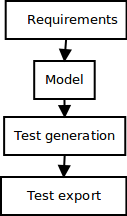
\includegraphics[scale=0.6]{figures/conformiq_process.png}
\caption{MBT process in Conformiq}
\label{fig:conformiq_process}
\end{figure}

\begin{enumerate}
	\item First step is specifying requirements. Conformiq support a huge amount of industrial requirements modelling tool (eg. IBM Rational, Rhapsody, Sparx Systems Enterprise, ArchitectHP Quality Center, IBM RequisitePro, DOORS), but it contains an own editor too. The defined requirements are traceable through the whole software testing process.
	\item Based on the requirements one has to create the model of the SUT. It can be done with the Conformiq Designer internal model editor using its QML language. The language consists three parts: system block diagrams, which describes the interface of the model (inbound and outbound ports); UML statecharts and Java like action language.
	\item After the modelling phase abstract test cases can be generated. The generation starts with transforming the model to an intermediate Lisp model, that is used during the symbolic execution, which generates the use cases. The user is able to see coverage statistics and a traceability matrix based on the generated test cases.
	\item Abstract test cases have to be exported with so called scripting backend which creates concrete test cases for the SUT.
\end{enumerate}

% section conformiq (end)

\section{GOTCHA}
\label{sec:gotcha}

GOTCHA is a framework that consist of two main components. The first one generates test cases from FSM models, while the others transforms abstract test cases into concrete test cases written in Java and then executes them on the SUT.

The model is described with GDL (GOTCHA Definition Language), that contains states, state variables, actions, expected results and guards. Abstract test cases are generated into XML format. Concrete test cases are executed on the SUT using an adapter, that can be written with the help of some helper class. The concrete method mapping is made by an XML file, that maps to specific SUT methods.

% section gotcha (end)

\section{ParTeG}
\label{sec:parteg}

Partition Test Generator is an open source Eclipse plugin, that can generate test cases from UML models annotated with OCL guards. It traverse the graph representing the UML state machine and each path corresponds to a test case.

The used test case generation algorithm is the following:

\begin{enumerate}
	\item A selected coverage criterion is transformed into model specific test goals.
	\item Each test goal references a concrete element of the model.
	\item From each of these element a path to the model's initial state represents a test case given by the corresponding transitions.
	\item Backwards on the path, each guard becomes a constraint on the inputs, which will be the initial input parameters in the end.
\end{enumerate}

% section parteg (end)

\section{Conclusions}
\label{sec:conclusions}

After investigating five widely used MBT tools, we can draw some consequences. From our point of view the most important parts of their features are the used model notation and the test case (TC) generation methods, because these are the most crucial part of the design. I summarised the collected information in the Table~\cite{tab:toolsummary}.

\begin{table}[htb]
\begin{center}
\begin{tabular}{|l|l|l|l|}
\hline
	\textbf{Name of the tool} & \textbf{Model} & \textbf{Intermediate model} & \textbf{TC generation method}\\\hline
	GraphWalker & FSM & graph (GraphML) & search based, combinatorial, random\\\hline
	PyModel & FSM + Python & graph & search based, random\\\hline
	Conformiq & QML & Lisp (CQ$\lambda$) & symbolic execution\\\hline
	GOTCHA & EFSM & graph & BFS, DFS\\\hline
	ParTeG & UML + OCL & graph & DFS, symbolic execution\\
\hline
\end{tabular}
\end{center}
\caption{\label{tab:toolssummary} Summary of examined MBT tools}
\end{table}

\begin{itemize}
	\item The tools implement different coverage criteria, but even the most useful state and transition coverage are not fully supported by each of the tools. More difficult criteria are avoided, for example transition pair, sneak path, all path and scenario coverage.
	
	Transition pair coverage may be avoided because the few added value compared to a full transition coverage. Another reason can be, that depending on the actual model and test case generation algorithm this criterion can be hard to implement properly.
	
	Sneak path means a path that contains an accepted method, that should not be accepted. By a fully specified model each possible transition is represented, so that sneak path criterion is not applicable.
	
	Usage of scenario coverage results reasonable smaller test suite, then the other test selection criteria, but a transition coverage may replace this criterion.
	\item Script-flow criteria are rarely used techniques. Only a few of them supports guards, but even those do not report on their coverage. Simple criteria as model flow criteria are not so effective at finding faults, whereas complex criteria like script flow criteria help find different kind of faults. On the other hand complex criteria are also significantly expensive in terms of theoretical complexity.
	\item Requirement traceability are ignored by just all the available tools. This feature make the tools more useful, but does not effect the ability to find more errors. Tracing requirements is rather used by software validation.
	\item Scaffolding solutions of the tools are incomplete. Fully automatic generation of test adaptors, oracles are seldom supported. These features make the testing tool more useful, because they accelerate the testing process.
	\item Regression tests are not supported. When an actual error is found, then the SUT should be tested against the generated test suite and this process should be supported by the testing tool.
	\item Creators of these tools either try to use an UML like model or FSM (EFSM). FSM models are low level representations of the SUT, so implementing search based algorithms and graph traversal algorithms are relatively easy.
	
	When engineers choose to use model with UML with graph intermediate model, they can not support complex UML state chart elements, such as orthogonal regions, because these features are hard to integrate into a graph representation.
	\item The intermediate model is just always some kind of graph representations, because the test case generation algorithms are the easiest to implement using graph models (search based test case generation, coverage criteria).
	\item Only a few tools have an integrated solution to create models. Handling models correctly is an essential feature of model based testing tools, because an integrated model editor improves the testing process greatly. Testing is an iterative process, so contextual switching between model editor and testing tool results an overhead.
	\item Input models are not verified. Model based testing the same as other testing methods can only find discrepancies regarding their source. If the test model is not correct, then the tests will be ineffective. That's why that is also important to verify the input model, and to help the testing process it can be built into the testing framework.
\end{itemize}

% section conclusions (end)

% chapter relatedwork (end)